\section{Kết quả Mô phỏng Thực nghiệm}

\subsection{Thực nghiệm cho ADE (Hình 2 \& Hình 3)}

\subsubsection{Thiết lập mô phỏng}

Dữ liệu được sinh từ mô hình với \(f^*\) là hàm phi tuyến trơn của \(D_t, X_t, H_t\). Tất cả các bộ dự đoán học máy (\(\hat{f}, \hat{m}\)) đều sử dụng Random Forest với tham số mặc định, được train trên tập phụ trợ độc lập cỡ \(T\). Thực nghiệm so sánh bộ ước lượng đề xuất \textbf{DML4SSI} với bốn phương pháp đối sánh:

\begin{itemize}
    \item \textbf{HT (Horvitz-Thompson):} Ước lượng hiệu số trung bình thông thường, hoàn toàn bỏ qua \(H_t\).
    \item \textbf{Plug-in:} Dùng học máy dự đoán trực tiếp kết quả, thiếu cơ chế debiasing.
    \item \textbf{Naive DML:} Áp dụng DML (AIPW) truyền thống, giả định i.i.d.\ và bỏ qua \(H_t\) trong mô hình kết quả.
    \item \textbf{SSAC (Shared State As Covariate):} Coi \(H_t\) như covariate độc lập thông thường; ước lượng điểm giống DML4SSI nhưng bộ ước lượng phương sai bỏ qua tự tương quan chuỗi thời gian.
\end{itemize}

\subsubsection{Kết quả}

\begin{figure}[H]
    \centering
    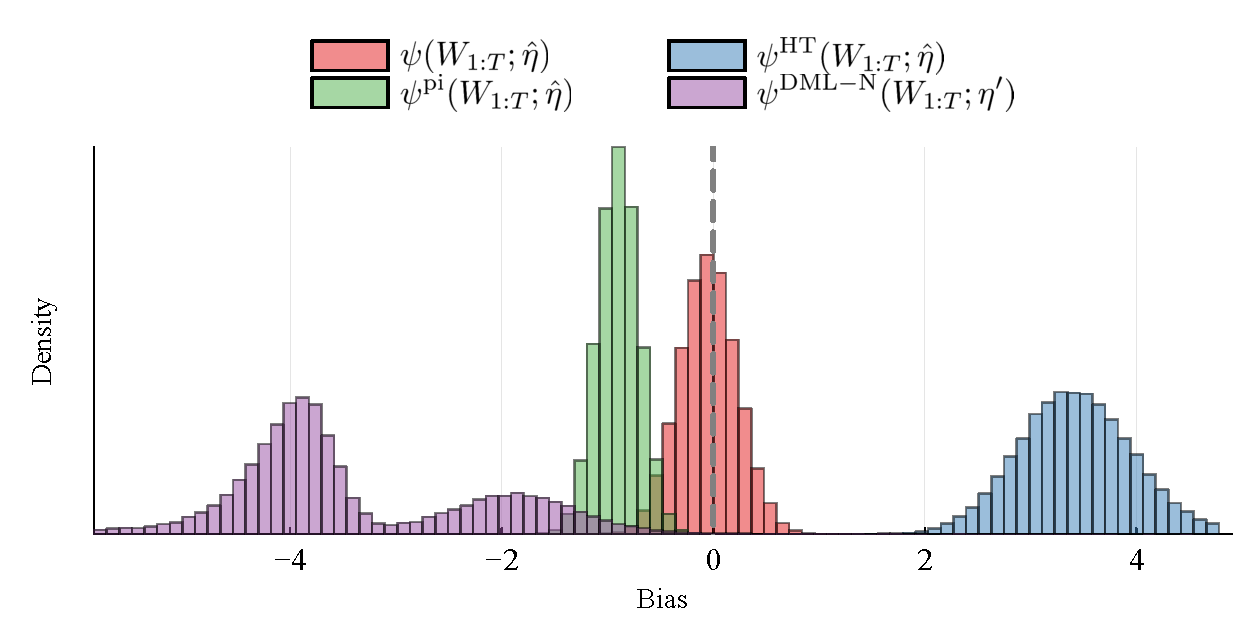
\includegraphics[width=0.65\textwidth]{image/direct_effect.pdf}
    \caption{Hình 2 --- Phân phối ước lượng điểm của ADE. Các phương pháp bỏ qua \(H_t\) (HT, Plug-in, Naive DML) bị chệch nặng; chỉ DML4SSI và SSAC tập trung quanh vạch 0 (giá trị thực).}
    \label{fig:ade_bias}
\end{figure}

\begin{figure}[H]
    \centering
    \begin{minipage}[t]{0.48\textwidth}
        \centering
        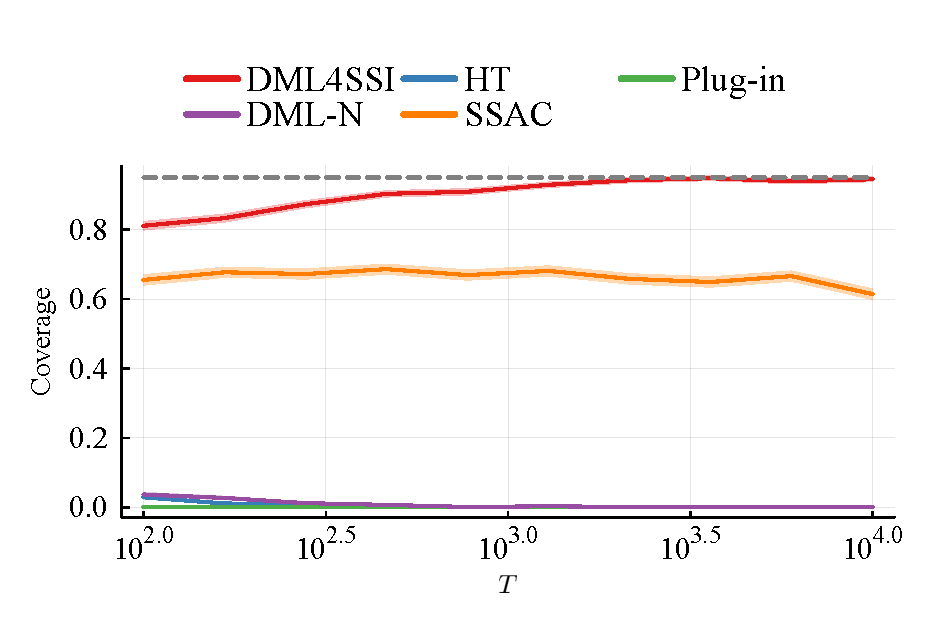
\includegraphics[width=\textwidth]{image/coverage_vs_sample_size.pdf}
    \end{minipage}
    \hfill
    \begin{minipage}[t]{0.48\textwidth}
        \centering
        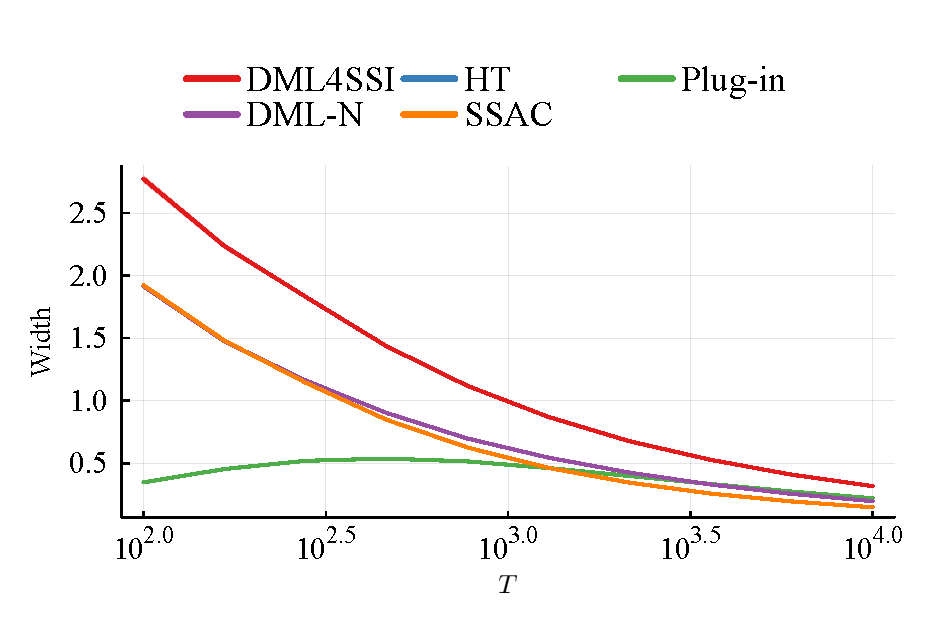
\includegraphics[width=\textwidth]{image/width_vs_sample_size.pdf}
    \end{minipage}
    \caption{Hình 3 --- Độ phủ (trái) và Độ rộng (phải) của khoảng tin cậy 95\% cho ADE theo cỡ mẫu \(T\). Chỉ DML4SSI hội tụ đến mức phủ chuẩn 95\%; SSAC bị kẹt ở 60--70\% do đánh giá thấp phương sai.}
    \label{fig:ade_ci}
\end{figure}

\begin{itemize}
    \item \textbf{DML4SSI:} Độ phủ nhanh chóng hội tụ về mức chuẩn \textbf{95\%} khi \(T\) tăng.
    \item \textbf{SSAC:} Tuy không chệch về điểm ước lượng nhưng \textbf{đánh giá thấp phương sai} do bỏ qua hiệp phương sai chuỗi thời gian --- khoảng tin cậy quá hẹp, độ phủ thực tế chỉ đạt 60--70\% và \textit{không bao giờ} hội tụ về 95\% dù tăng \(T\).
    \item Các phương pháp naive (HT, Plug-in, Naive DML): độ phủ xấp xỉ 0.
\end{itemize}

\textbf{Kết luận:} Chỉ \textbf{DML4SSI} đồng thời đảm bảo ước lượng điểm không chệch \textit{và} khoảng tin cậy đạt mức phủ chuẩn 95\%.

\subsection{Thực nghiệm cho GATE trong Switchback (Hình 4, 5 \& 6)}

\subsubsection{Thiết lập mô phỏng}

Tương tự phần ADE, với \(f^*\) là hàm phi tuyến của \(D_t, X_t, H_t\) và độ dài switchback \(\ell = 2m\). Bộ ước lượng đề xuất được so sánh với:

\begin{itemize}
    \item Các phương pháp naive (HT, Plug-in, Naive DML) --- như trong bài toán ADE.
    \item \textbf{Switchback HT (SB)} (Bojinov et al., 2022): bộ ước lượng không chệch được thiết kế đặc biệt cho thử nghiệm switchback.
\end{itemize}

\subsubsection{Kết quả}

\begin{figure}[H]
    \centering
    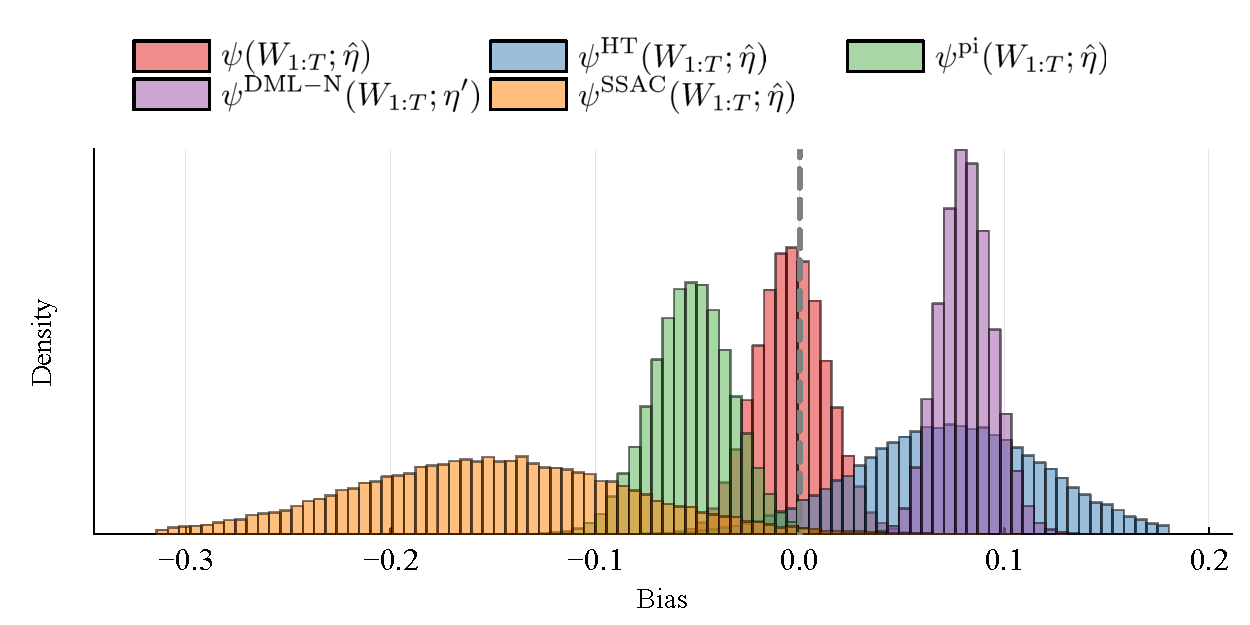
\includegraphics[width=0.65\textwidth]{image/switchback_vs_naive.pdf}
    \caption{Hình 4 --- Phân phối ước lượng điểm của GATE trong Switchback: DML4SSI so với các phương pháp naive. Các phương pháp naive bị chệch nặng; DML4SSI tập trung xung quanh giá trị thực.}
    \label{fig:gate_bias}
\end{figure}

\begin{figure}[H]
    \centering
    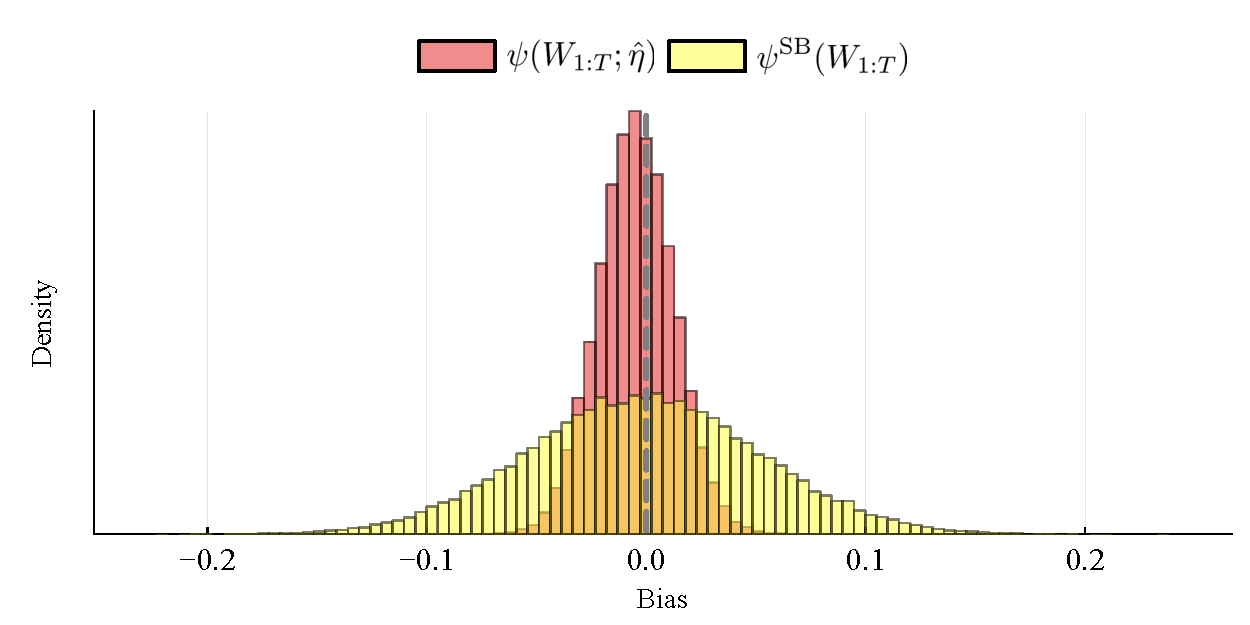
\includegraphics[width=0.65\textwidth]{image/switchback.pdf}
    \caption{Hình 5 --- So sánh DML4SSI với Switchback Horvitz-Thompson (SB). Cả hai đều không chệch nhưng DML4SSI có phương sai thấp hơn đáng kể (phân phối nhọn hơn).}
    \label{fig:gate_vs_sb}
\end{figure}

Cả hai phương pháp đều \textit{không chệch} (phân phối cân tâm tại giá trị thực), nhưng \textbf{DML4SSI có phương sai thấp hơn đáng kể}. Hai lý do chính:
\begin{enumerate}
    \item Học máy giải thích biến động qua covariate và trạng thái chung, loại bỏ nhiễu không cần thiết.
    \item Phương pháp SB bắt buộc phải bỏ đi \(m\) bước đầu mỗi khối chuyển giao, trong khi DML4SSI tận dụng toàn bộ dữ liệu thông qua thành phần Regression Adjustment.
\end{enumerate}

\begin{figure}[H]
    \centering
    
\includegraphics[width=0.75\textwidth]{image/gate_coverage_width.png}
    \caption{Hình 6 --- Độ phủ (trái) và Độ rộng (phải) của khoảng tin cậy 95\% cho GATE theo cỡ mẫu \(T\). DML4SSI hội tụ về 95\%; SB đạt 100\% do phương sai ước lượng quá bảo thủ, dẫn đến khoảng tin cậy rộng hơn DML4SSI từ 3 đến 7,5 lần.}
    \label{fig:gate_ci}
\end{figure}

\begin{itemize}
    \item \textbf{Độ phủ (Coverage):} DML4SSI nhanh chóng hội tụ về mức chuẩn 95\%. SB luôn đạt 100\% do ước lượng phương sai quá bảo thủ.
    \item \textbf{Độ rộng (Width):} Khoảng tin cậy của SB \textbf{rộng gấp 3 đến 7,5 lần} so với DML4SSI.
\end{itemize}

\textbf{Ý nghĩa kinh tế:} Khả năng thu hẹp khoảng tin cậy của DML4SSI cho phép doanh nghiệp \textbf{tiết kiệm 3--7,5 lần cỡ mẫu hoặc thời gian chạy A/B test} để đưa ra quyết định với cùng mức độ tin cậy.
